\section{Praktikos veiklos aprašymas}

\subsection{Projektas}
Kaip buvo minėta ankščiau, profesinės praktikos metu visi darbai buvo vykdomi su „Bitė Lietuva“ vidinė klientų aptarnavimo informacinė sistema.
„Bitė Lietuva“ yra įmonės nuolatinis klientas, 2018 metais „INVENTI“ sukūrė šią sistemą \cite{medus}, ir integravo su egzistuojančiomis „Bitė Lietuva“ sistemomis.
Sistema įmonės viduje turi kodinį pavadinimą „medus“ \ref{img:medus}.
Klientui „Bitė Lietuva“ atsirado poreikis atlikti televizijos paslaugų pardavimą per šią sistemą, tam kad galutinis vartotojas galėtų naudotis
„Go3 | BITĖ“ televizijos paslaugomis \cite{go3}. „INVENTI“ pasirašė sutartį atlikti šį projektą dviem etapais.
Taip pat prie projekto prisijungė ir kiti vendoriai - įmonė „Baltic Amadeus“. Šio darbo rašymo metu šalyje yra paskelbtas karantinas, dėl koronaviruso
COVID-19 grėsmės. Atsižvelgiant į tai, „Bitė Lietuva“ siūlo televizijos paslaugomis 3 mėnesius naudotis nemokamai.


\begin{figure}[H]
    \centering
    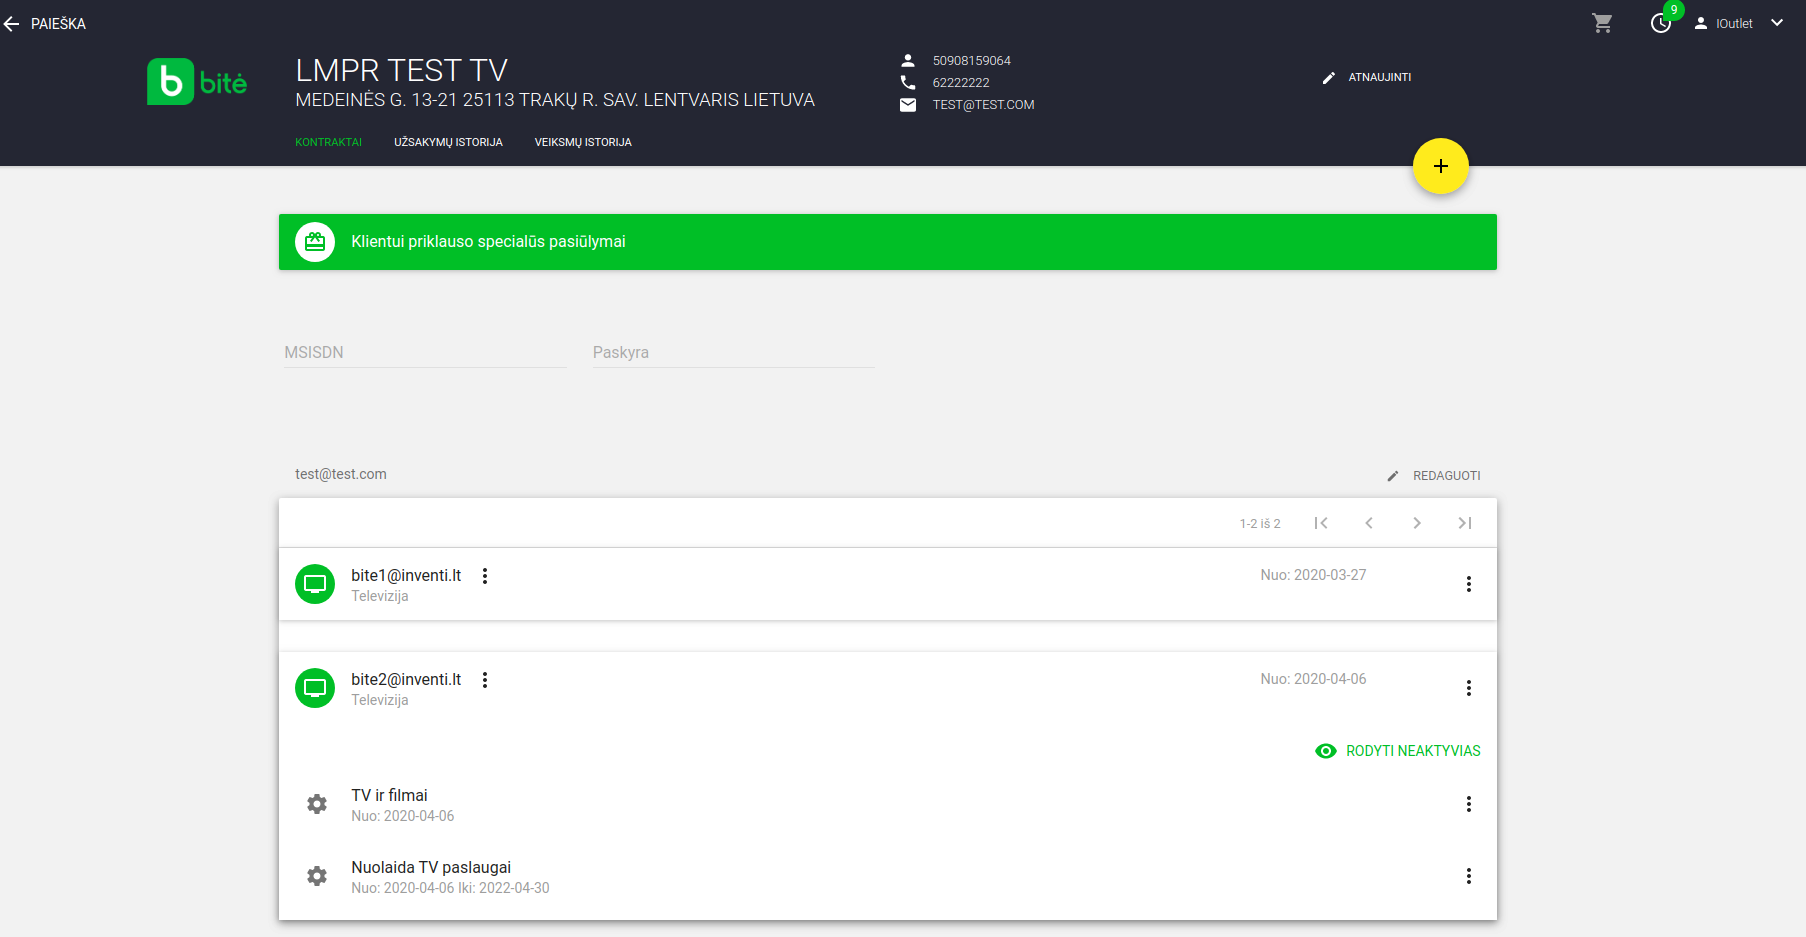
\includegraphics[scale=0.25]{img/medus.png}
    \caption{Vidinės klientų aptarnavimo sistemos vartotojo sąsaja.}
    \label{img:medus}
\end{figure}

\subsection{Darbo procesas}
Prieš pradedant projektą, komanda atlieka kliento pateiktų vartotojų istorijų analizę, išskaido jas į užduotis, kiekvieną užduotį įvertina, ir sudeda į projekto neatliktų užduočių sąrašą.
Darbas vykdavo pagal agile metodologiją, kas dvi savaites planuojami sprintai. Sprinto planavimo metu, visa komanda susirenka ir padaro atliktų užduočių apžvalgą „JIRA“
užduočių projekto sistemoje, apžvelgiama, kokios užduotys buvo atliktos praeitame sprinte, o kurios keliauja į naują.
Atlikus peržiūrą, praeitas sprintas uždaromas, atidaromas naujas. Neužbaigtos užduotys perkeliamos į naują sprintą, ir tada atliekama neatliktų užduočių sąrašo analizė.
Iš neatliktų užduočių sąrašo, užduotys perkeliamos į naują sprintą pagal svarbumo prioritetą, tol, kol nebus viršytas dviejų savaičių darbo valandų limitas. Įmonėje taikoma praktika,
kad programuotojas programavimo darbams vidutiniškai skiria 6 valandas, 2 valandos lieka susitikimams, pokalbiams su klientu, arba kitai, su programavimu nesusijusiai veiklai.
Pirmadieniais vykdavo susitikimas, kurio metu buvo uždaromas praeitas sprintas ir buvo planuojamas naujas.

Kiekviena diena ryte vyksta „stand-up“ susitikimai, dažniausiai tai skambutis su klientu ir kitais vendoriais, bet kartais tekdavo vykti pas klientą į ofisą, kur šie
susitikimai vykdavo gyvai. Kiekvienas „stand-up“ dalyvis trumpai nupasakoja, ką praeitą dieną nuveikė, su kokiomis problemomis susidūrė ir kaip jas sprendė.
Šie susitikimai dažniausiai užtrunka 15 minučių, po jų seka komandos vidiniai komandos pasitarimai.




\subsection{Projekte naudojamos technologijos}

Sistemos UI dalis yra parašyta su JavaScript kalba,
naudojama „React“ biblioteka. Sistemos serverinė dalis parašyta su Java programavimo kalba, naudojamas „Spring“ programavimo karkasas. Serverinė dalis yra išskaidyta į
posistemes, šis išskaidymas yra mikroservisų (angl. „microservices“) architektūrinis principas. Servisai tarpusavyje apsikeičia duomenimis per
REST (angl. „Representational State Transfer“) arba SOAP (angl. „Simple Object Access Protocol“) sąsają. Taip pat tam tikri servisai įgyvendina
CQRS (angl. „Command Query Response Segregation“) architektūrinį principą, kuris atskiria duomenų įrašymo ir duomenų užklausų sluoksnius.
